%Chapter 3

\chapter{Représentation sémantique d'images} % Main chapter title

\section{Introduction}
	Dans ce chapitre nous allons présenter nos différentes approches pour la réalisation d'une recherche d'image par le contenu (CBIR) basée exemple. Contrairement aux techniques traditionnelles qui utilisent les formes, textures, couleurs, etc. pour comparer les images (calculer la ressemblance), nous allons utiliser dans nos approches des techniques de l'apprentissage profond. Parmi les techniques d'apprentissage profond auxquelles nous allons nous intéresser se trouvent les réseaux à convolution (ConvNets) et les Deep AutoEncoders. 
	
	Nos premières tentatives consisteront en l'exploration de différentes méthodes permettant d'extraire la description d'une image à partir d'un réseau à convolution. Puis nous allons essayer réduire cette description vers un espace de représentation plus petit à l'aide des Deep Autoencoders, et observer ce que cette réduction apporte en terme de performance. Enfin, nous introduirons des descripteurs de textures à nos descriptions extraites par les technique d'apprentissage profond et constater si cela apporte des améliorations dans l'extraction des images ressemblantes. Nous allons aussi donner pour chacune de nos approches, des interprétations bien fondées des différents résultats que nous avons obtenus, ainsi qu'une étude comparative avec des systèmes connus de recherche d'images par le contenu qui utilisent les descripteurs d'images traditionnels.
	
	


\section{Recherche d'images par le contenu basée exemple}
	Parmi les types de la recherche d'images par le contenu mentionnés au chapitre 1, nous avons choisi celui basée-exemple pour sa facilité d'implémentation. Notre algorithme de recherche d'image par le contenu basée exemple nécessite une grande base d'images, pour cela nous avons utilisé deux bases différentes, la première est celle de WANG [Wan et al.,01][Li et Wan.,03] contenant 1000 images (10 classes de 100 images) [Figure 3.1].

\begin{figure}[H]
	\centering
		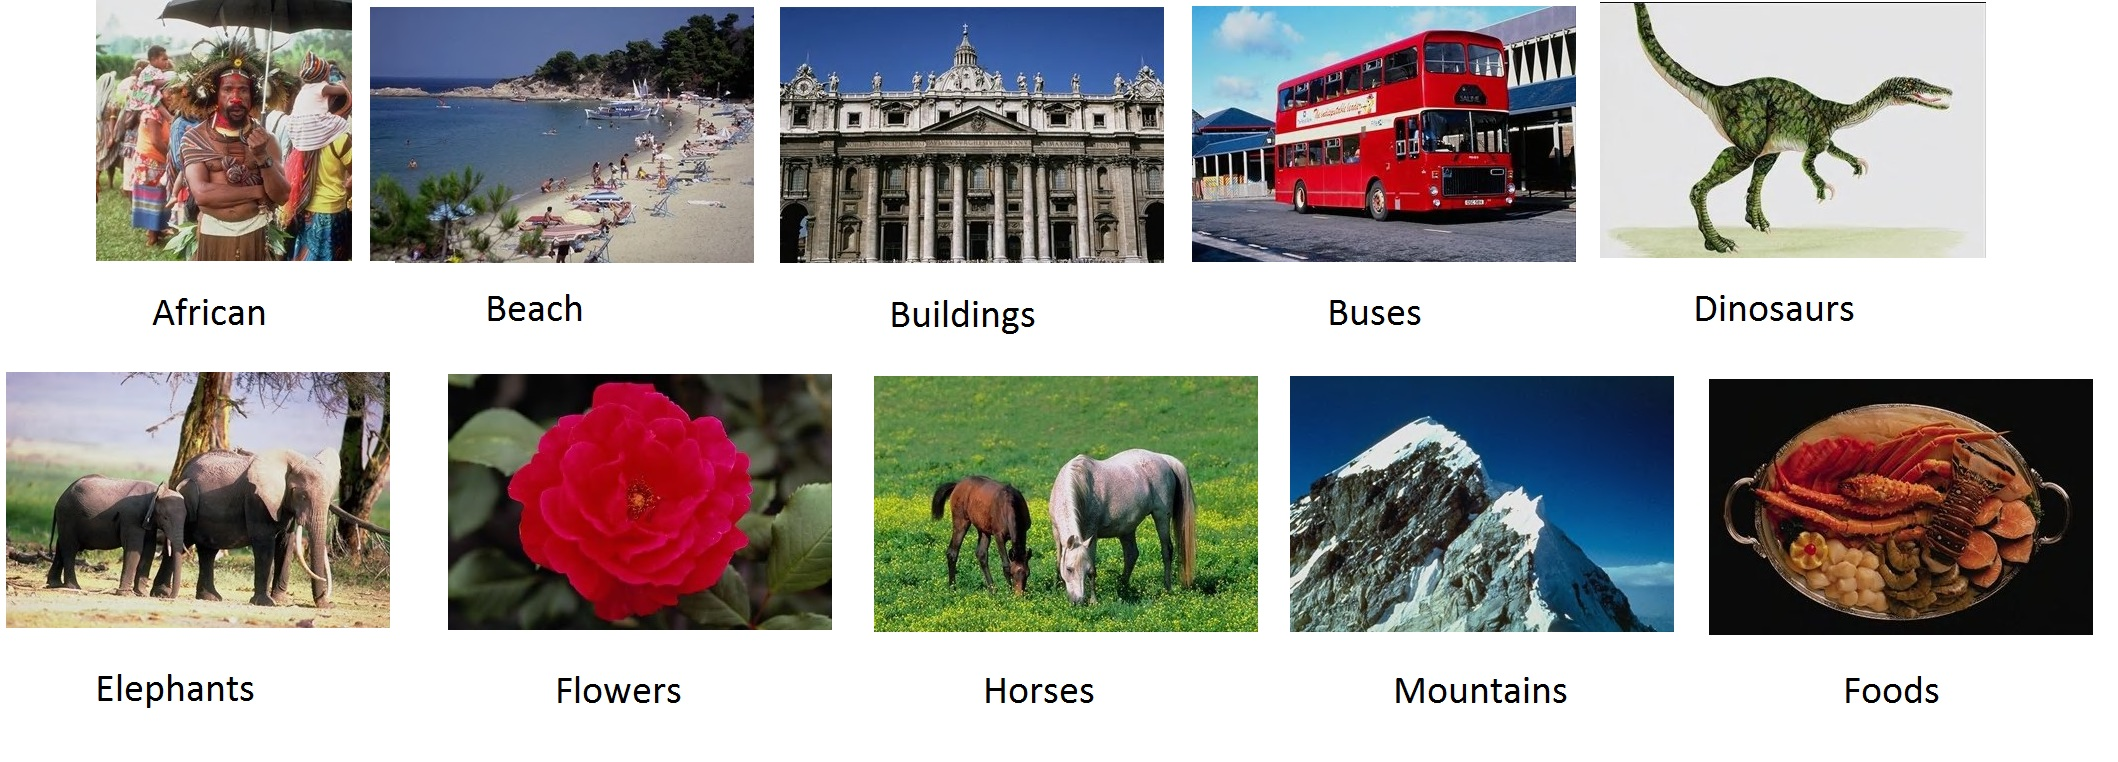
\includegraphics[width=7in]{Figures/wang.jpg}
	\caption[An Electron]{Exemples d'image de la base WANG.}
	\label{fig:Electron}
\end{figure}

	La deuxième est Caltech101 (100 classes) [Fei et al. 04] contenant plus de 9000 images [Figure 3.2]. Nous avons choisi ces deux bases d'images pour la simple raison que les images sont déjà classées (une unique classe par image), ce qui facilitera le calcul des mesures de performance, on pourra donc vérifier facilement si deux images appartiennent à la même classe.
	


\begin{figure}[H]
	\centering
		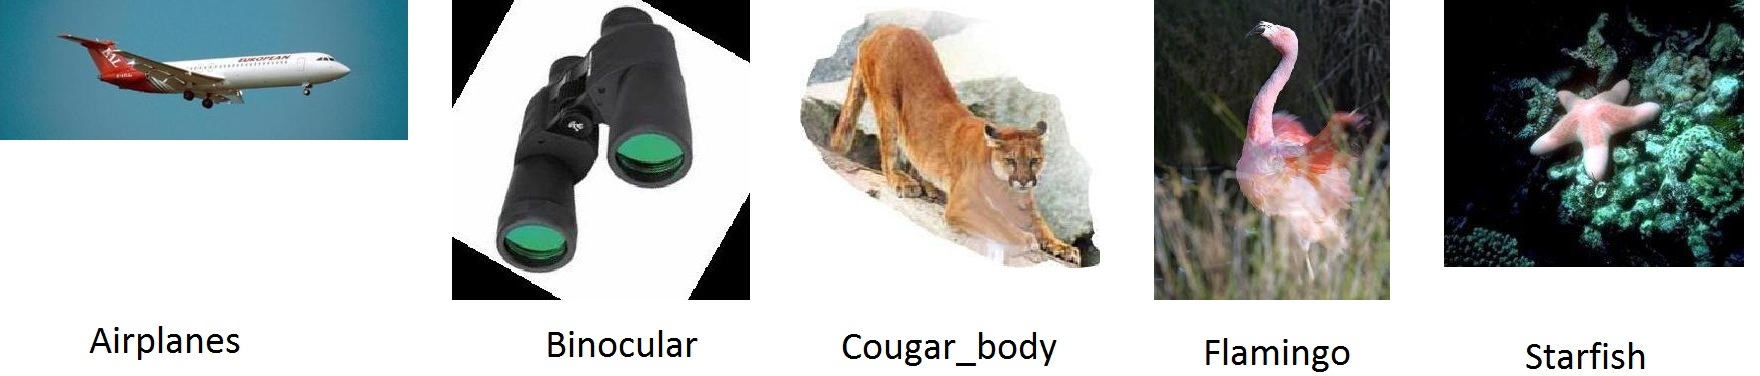
\includegraphics[width=5.6in]{Figures/caltech101.jpg}
	\caption[An Electron]{Exemples d'image de la base Catlech-101.}
	\label{fig:Electron}
\end{figure}	
	
	
	Afin de comparer nos différentes approches, nous allons calculer pour chacune les mesures de performance obtenues. Pour cela nous allons appliquer notre algorithme de recherche d'image par le contenu basée-exemple comme suit:


\begin{algorithme}[H]
\caption{Recherche d'images par le contenu basée exemple}
\Function{CBIR}
{\textit{Base}: \textbf{Base d'images}, \textit{Comp}: \textbf{Approche de Comparaison}}{Mesures de performance}
{
\begin{enumerate}


\item Diviser \textit{Base} en deux parties:
\begin{enumerate}[a]
\item \textit{Query}: Extraire aléatoirement de chaque classe de \textit{Base} 20\% d'images.
\item \textit{Test}: Les 80\% restantes.
\end{enumerate}

\item \For {chaque classe \textit{C} de \textit{Query}}
{
\begin{enumerate}
\item \For {chaque image $\textit{Q}\in\textit{C}$ de \textit{Query}}
{
	\begin{enumerate}[a]
	\item \For {chaque image \textit{T} de \textit{Test}}
	{
		Calculer la ressemblance \textit{R} entre \textit{Q} et \textit{T} avec l'approche 
		
		\textit{Comp}.
	}
	\item \textit{Resemb} = liste des images de \textit{Test} triées selon \textit{R} par ordre 
	
	
	décroissant.
	\item Comparer la classe \textit{C} de \textit{Q} avec les classes des images 
	
	triées \textit{Resemb}
	\item Calculer les mesures de performance \textit{Perf}.
	\end{enumerate}
}
\item Calculer la moyenne des mesures de performance de \textit{C}.
\end{enumerate}
}
\item Retourner la moyenne des mesures de performance Totale.
\end{enumerate}
}
\end{algorithme}

	La première étape de notre algorithme est de diviser une base contenant plusieurs images en deux parties: Nous appellerons la première \textit{Query}, contenant 20\% des images (choisies aléatoirement) qui seront utilisées en tant que requêtes. Les 80\% des images restantes seront dans la deuxième partie que nous appellerons \textit{Test}.

	Notre but étant que pour chaque image requête de \textit{Query}, nous allons trouver les images qui lui ressemblent le plus de la partie \textit{Test}. Nos méthodes de comparaison (calcul de ressemblance) entre les images ce feront avec plusieurs approches que nous allons présenter plus bas.

	En ayant la liste des images les plus ressemblantes à une requête donnée triée par ordre décroissant (de l'image la plus ressemblante à la moins ressemblante), et pour comparer nos différentes approches que nous avons réalisé, nous devons calculer les mesures de performance qui sont comme suit : 
\begin{enumerate}

\item \textbf{Précision à 1}: 1-Précision, elle est égale à 100\% si l'image la plus ressemblante à la requête qui est retournée par l'approche est effectivement de la même classe que l'image en entrée, et 0\% dans le cas contraire.
\item \textbf{Précision à \textit{N}}: ou N-Précision \textit{N} étant un nombre d'images (5,10,20,40 ou 60). Cette mesure donne le pourcentage d'images  pertinentes (qui appartiennent à la même classe que l'image requête), parmi les \textit{N} images les plus ressemblantes retrouvées par l'algorithme.
$$N-Précision = \frac{Nombre des images pertinentes retrouvées}{Nombre N des images retrouvées}$$
\item \textbf{Rappel}: C'est le pourcentage d'images  pertinentes, parmi le nombre total des images pertinentes (les images qui appartiennent réellement à cette classe).
$$R = \dfrac{Nombre des images pertinentes retrouvées}{Nombre total des images pertinentes}$$
\item \textbf{Taux d'erreur}: C'est l’événement contraire de la 1-Précision.
$$Taux d'erreur = 1 - \textit{1-Précision}$$


%$$ N-précision = \dfrac{images réelement pertinentes top-N}{N} Rappel = \dfrac{Img Per}{N}$$

\end{enumerate}

	Contrairement à la base d'images WANG, nous avons remarqué que les classes de la base Caltech101 (101 classes) ont un nombre d'images qui est différent entre chaque classe, nous allons donc d'abord calculer les moyennes de performance d'une classe donnée, ensuite calculer la moyenne des performances totale de l'approche. Comme ça les classes ayant un nombre très grands (très petits) d'images, ne seront pas plus avantagées (moins avantagées) par rapport aux autres classes.

	
\section{Architecture du réseau à convolution}
	Comme nous l'avons cité précédemment, notre approche utilisera des techniques d'apprentissage profond pour la comparaison des images à la place des techniques traditionnelles (texture, forme, couleur, etc.). Pour cela, nous avons utilisé les réseaux à convolution (ConvNets) introduits dans le chapitre précédent.
	
	L'architecture VGG-CNN-S du réseau à convolution que nous avons utilisé dans notre algorithme, a été proposée par l'équipe de recherche Visual Geometry Group Department of Engineering Science, Université d'Oxford (VGG) [Cha et al.14]. Lors de la compétition ImageNet 2014 (introduite au chapitre 2) ils ont pu obtenir une erreur de classification (top-5) de 7.405\%. L'architecture VGG-CNN-S du ConvNets a été entraînée sur une base d'images très grande ILSVRC-2012 (plus de 1.2 millions d'images [Rus et al.15]). Cette base contient 1000 classes différentes, elle inclut une très grande variété d'images et a donc beaucoup de potentiel pour être généralisable, c’est-à-dire elle peut donner aussi de bons résultats sur d'autres bases d'images qui sont plus petites que celles de ILSVRC-2012.
	
	Nous allons donc commencer par décrire l'architecture VGG-CNN-S du réseau à convolution que nous avons utilisée. Le tableau ci-dessous donne une descriptions de chacune des couches de l'architecture du ConvNets utilisé qui est comme suit:

\begin{table}[H]
\begin{center}
\begin{tabular}{|c|c|c|c|c|c|c|c|}
\hline
ConvL & ConvL & ConvL & ConvL & ConvL & FC-MLP & FC-MLP & FC-MLP\\
  \hline
96x7x7 & 256x5x5 & 512x3x3 & 512x3x3 & 512x3x3 & 4096 & 4096 & 1000\\
st. 2,pad 0 & st. 1,pad 1 & st. 1,pad 1 & st. 1,pad 1 & st. 1,pad 1 & drop- & drop- & soft-\\
LRN,x3 pool & x2 pool & - & - & x3 pool & out & out & max\\
  \hline
\end{tabular}
\end{center}
\caption{Architecture de VGG-CNN-S [Cha et al.14].}
\caption*{
    Légende:
    \begin{tabular}{l l}
      ConvL & Couche de pile de convolutions \\
      FC-MLP & Perceptron multicouche entièrement connecté\\
    \end{tabular}
  }
\end{table}

	Ce réseau à convolution comporte une couche d'entrée (non incluse dans le tableau), 7 couches cachées et une couche de sortie (la dernière colonne du tableau). Les données en entrée au réseau à convolution sont des images ayant une taille fixe de 224 x 224 pixels RGB. Pour forcer cette taille à toutes les images, elles seront d'abord redimensionnées de telle sorte à ce que la plus petite des deux dimensions (longueur ou bien largeur) soit égale à 256 pixels, ensuite on prendra les 224 x 224 pixels qui sont au centre de ces images. Le choix de la valeur de 224 pixels est nécessaire pour que les données en entrée s'adaptent à l'architecture proposée. Le seul pré-traitement effectué est la soustraction de la valeur moyenne RGB de chaque pixel de l'image, son interprétation géométrique est de centrer le nuage de données autour d'une origine [CS231n 16].

	L'image passe premièrement à travers des piles de couches de convolution où nous appliquons plusieurs filtres. La première couche de convolution applique 96 filtres différents de taille $7x7$ pixels avec un stride de 2 et sans zero-padding, comme le montre la figure suivante:

\begin{figure}[H]
	\centering
		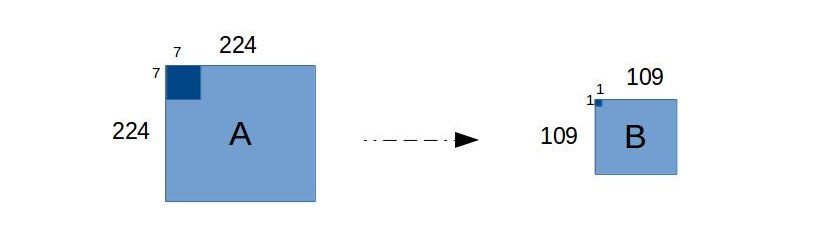
\includegraphics[width=7.5in]{Figures/conv.jpg}
	\caption[An Electron]{Application d'un filtre de convolution.}
	\label{fig:Electron}
\end{figure}

	La valeur du stride représente le nombre de pixels de déplacement d'un filtre sur une image après chaque opération de convolution. Le passage d'une image à travers une pile de convolution aura pour effet de changer la dimension (nombre de pixels) de l'image. Posons $S$ la valeur du stride, $P$ la valeur du zero-padding, $W_{1}$ le nombre de pixels d'une dimension (longueur ou bien largeur) d'une image et $F$ la taille des filtres de convolution. Pour calculer la taille obtenue en sortie $W_{2}$, on applique la formule suivante:
$$W_{2} = (W_{1} - F + 2*P)/S + 1$$
$$Exemple de la première convolution: (224 - 7 + 2*0)/1 +1 = 109.5$$
	
	Si on obtient un nombre non entier (avec une virgule) comme l'exemple ci-dessus, ce qui représente une opération de convolution incomplète, on ne prend alors que la partie entière. Comme les images en entrée ont la même largeur et longueur (images carrées), il suffit seulement de calculer cette valeur (nouvelle dimension) pour une seule dimension.
	Cette première couche de convolution est la seule couche sur laquelle on applique une normalisation [Kri et al.,12].
	
	Après cela, on applique un max-pooling sur la sortie résultante des convolutions, comme le montre la figure suivante:

\begin{figure}[H]
	\centering
		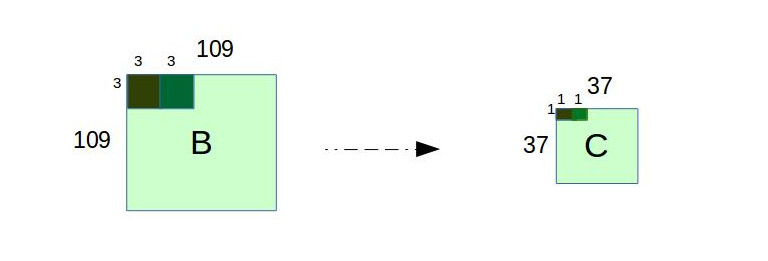
\includegraphics[width=7in]{Figures/pool.jpg}
	\caption[An Electron]{Application d'un max-pooling.}
	\label{fig:Electron}
\end{figure}

	En posant $W_{1}$ le nombre de pixels d'une dimension d'une image, $F$ la taille du max-pooling et $S$ la valeur du stride qui est égale à $F$. On peut calculer la taille du résultat $W_{2}$, comme suit:

$$W_{2} = (W_{1} - F )/S + 1$$
Exemple du premier max-pooling: $$(109 - 3)/3 +1 = 36.33$$

	Ces étapes sont presque les mêmes pour chaque couche de convolution, chacune applique des filtres de convolution d'une certaine taille, suivis ou non d'un max-pooling. On remarque sur la figure qui va suivre dans la troisième couche de convolution, que la taille de l'entrée est de 17x17 et de la sortie 17x17, comme on a dit dans le chapitre précédent cela est dû au zero-padding qui permet de contrôler la dimension des sorties. On remarque aussi que la plus petite taille des filtres de convolution est de 3x3 pixels, et cela pour capturer la notion de gauche / droite, haut / bas, au centre.

	Les sorties obtenues après le passage d'une image sur ces couches de convolutions sont 512 matrices de taille 6x6 pixels, 512 étant le nombre de filtres appliqués lors de la dernière convolution, et la taille 6x6 pixels est la taille de la sortie de cette même couche après application des filtres de convolution et du max-pooling.

	L'empilement des couches de convolution est suivi par trois couches (les 3 dernières couches du tableau) entièrement connectées (Fully-Connected Layers), pour faire passer en entrée les valeurs des sorties des convolutions on devra aplatir les matrices obtenues précédemment (521 matrices de 6x6 pixels) en un seul vecteur unidimensionnel.
	
	La figure suivante montre comment plusieurs matrices seront aplaties en un seul grand vecteur à une seule dimension:

\begin{figure}[H]
	\centering
		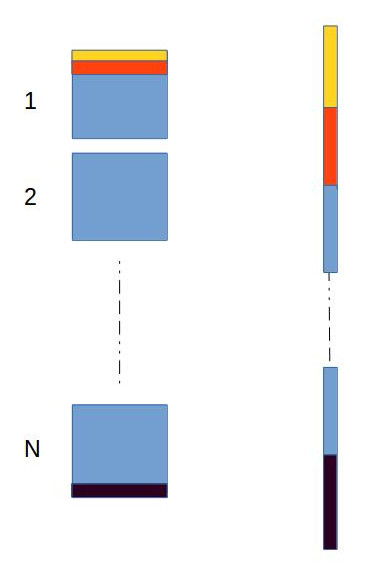
\includegraphics[width=3.5in]{Figures/flattening.jpg}
	\caption[An Electron]{Applatissement des résultats du ConvNets.}
	\label{fig:Electron}
\end{figure}

	Le vecteur unidimensionnel sera composé de la succession des lignes de la première matrice, ensuite les lignes de la deuxième matrice, et ainsi de suite jusqu'à la dernière matrice. Donc dans notre cas, à partir de 512 matrices de 6x6 nous aurons un vecteur unidimensionnel de taille: $512*6*6 = 18432$.

Les deux premières couches entièrement connectées ont 4096 neurones chacune, la troisième et dernière couche du réseau est la couche soft-max. Elle réalise la classification de la base d'images ILSVRC-2012 et contient donc 1000 neurones (un pour chaque classe), cette couche soft-max donnera comme sortie un vecteur de 1000 valeurs contenant les probabilités d'appartenance d'une image aux 1000 classes.

	La figure suivante montre l'architecture complète contenant la taille de chaque entrée et sortie de chaque couche du réseau à convolution:

\begin{figure}[H]
	\centering
		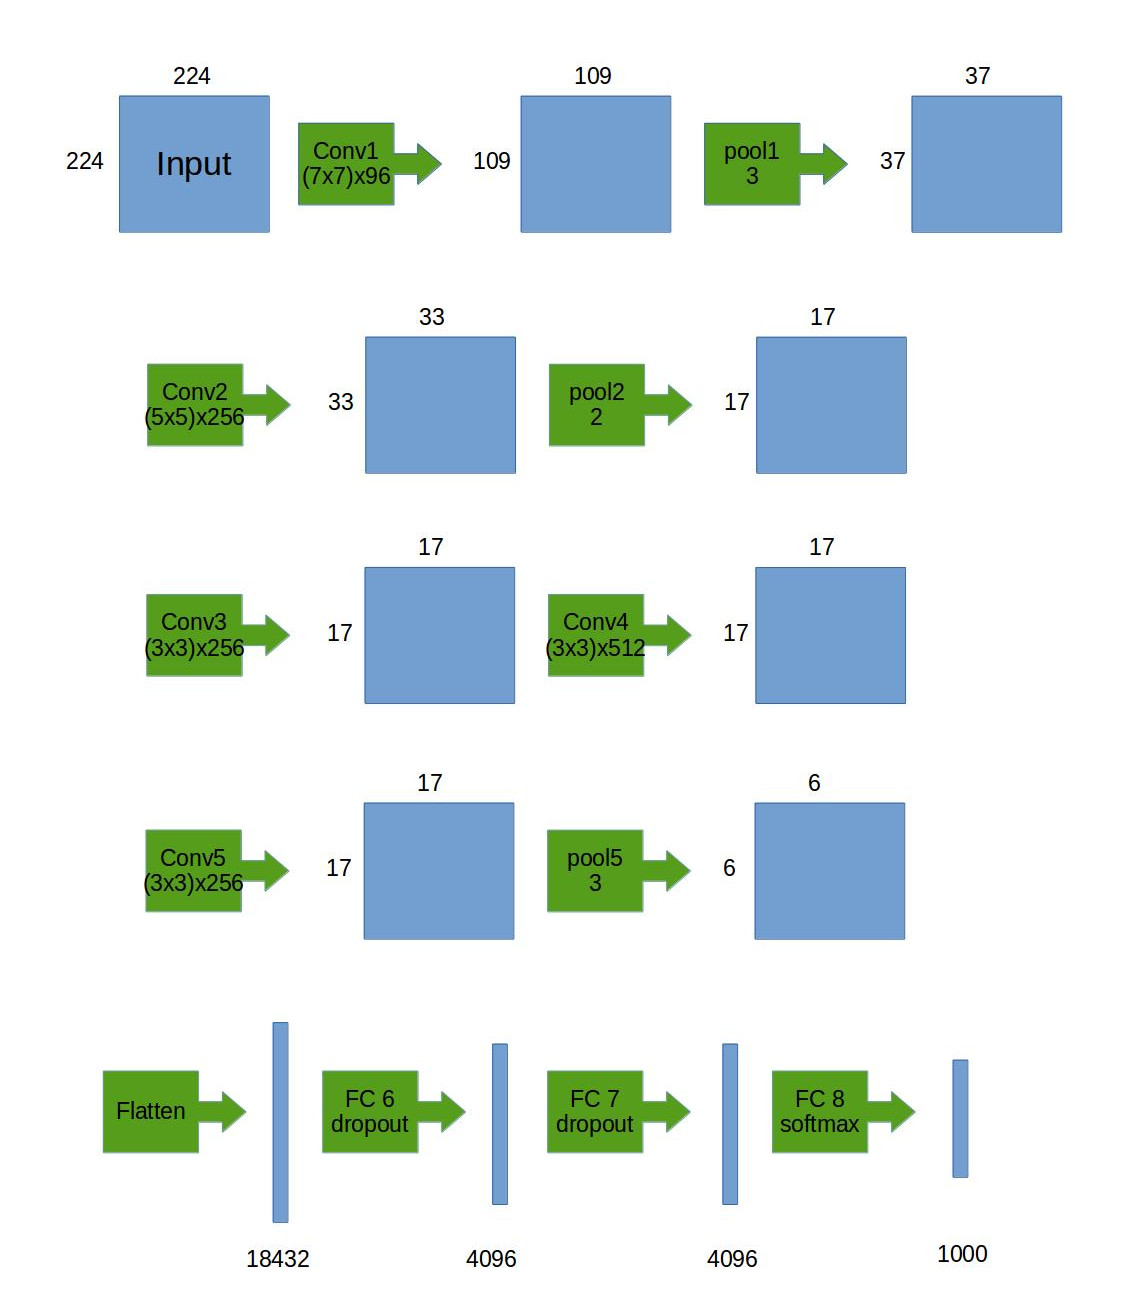
\includegraphics[width=6in]{Figures/architectureVGG.jpg}
	\caption[An Electron]{Architecture complète du ConvNets.}
	\label{fig:Electron}
\end{figure}



\section{Entraînement du réseau}
	Comme pour un réseau de neurones ordinaire, un réseau de neurones à convolution a besoin d'être entraîné sur une base d'exemples (base d'images dans notre cas), plus le réseau a une grande taille (plusieurs poids) plus on aura besoin d'un plus grand nombre d'exemples pour son entraînement. 
	
	La base utilisée pour l’entraînement (apprentissage) de ce réseau à convolution est ILSVRC-2012 (plus de 1.2 million d'images), et l'apprentissage s'est fait avec une descente du gradient stochastique avec moment. Les paramètres empiriques (hyper-paramètres) sont comme suit: Un moment de $0.9$, une dégradation des pondérations (weight decay) de $5*10^{-4}$, et un taux d'apprentissage initial (learning rate) de $10^{-2}$. [Cha et al.14]
	
	Les valeurs initiales des poids ne peuvent pas être toutes égales à zéro (ou une autre valeur), puisque tous les poids vont calculer le même gradient lors de la rétro-propagation, ce qui résultera en l'application des mêmes mis-à-jours sur tous les poids. En d'autres termes, il n'y aura pas d’asymétrie entre les valeurs des poids si elles sont toutes initialisées à une même valeur. [CS231n 16]	
	Il serait donc plus judicieux d'initialiser les valeurs des poids à des valeurs aléatoires proches de zéro. Pour l'architecture VGG-CNN-S, les valeurs des poids de chaque couche ont été initialisées avec une distribution Gaussienne avec une moyenne de 0 et une variance de $10^{-2}$. [Cha et al.14]
	
	Il est évident que pour réaliser l’entraînement d'un aussi grand réseau requiert de très grands temps de calculs et une très grande puissance CPU/GPU de calculs. L'équipe Visual Geometry Group a utilisé pour cela une carte graphique NVIDIA GTX Titan, l'entraînement du réseau à convolution a duré pendant 3 semaines, sans inclure le temps de paramétrage des hyper-paramètres (moment, learning rate, etc.).
	
	Comme dans notre cas, nous ne disposons pas d'une aussi grande puissance de calcul ni le temps nécessaire pour paramétrer le réseau à convolution, nous ne pouvons pas réaliser l’entraînement de ce réseau. L'équipe VGG a eu donc la courtoisie de publier pour les chercheurs les poids que leurs réseaux (VGG-CNN-S et autres) ont appris durant la phase entraînement, nous n'avons donc pas eu à refaire ce qui a été fait.
	
	Nos contributions à la recherche d'image par le contenu, peuvent être résumées sur les trois schémas suivant:
	
	\begin{figure}[H]
	\centering
		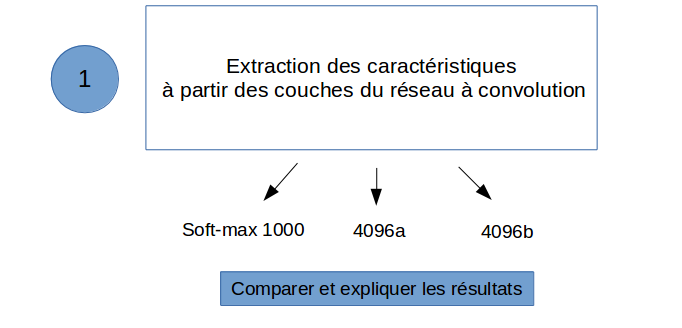
\includegraphics[width=5in]{Figures/diagramme1.png}
	\caption[An Electron]{Approches de l'extraction des caractéristiques.}
	\label{fig:Electron}
\end{figure} 

	\begin{figure}[H]
	\centering
		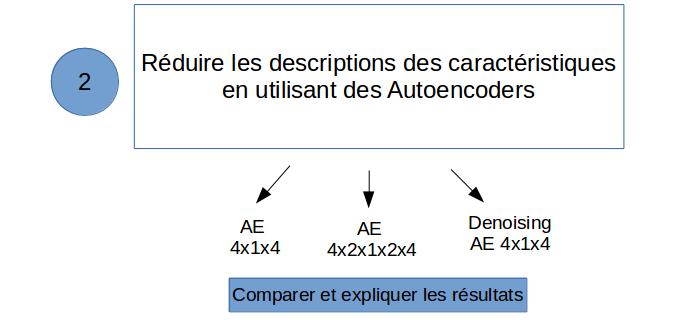
\includegraphics[width=5in]{Figures/diagramme2.png}
	\caption[An Electron]{Approches de la compression avec les Autoencoders.}
	\label{fig:Electron}
\end{figure} 

	\begin{figure}[H]
	\centering
		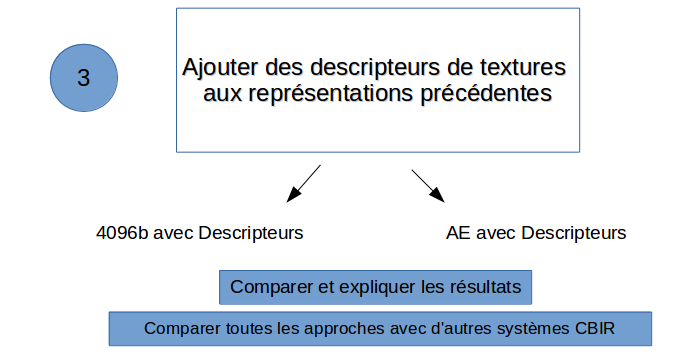
\includegraphics[width=6in]{Figures/diagramme3.png}
	\caption[An Electron]{Approches de l'ajout des descripteurs de textures.}
	\label{fig:Electron}
\end{figure} 

\section{Extraction des caractéristiques}
	L'architecture du réseau à convolution utilisée contient une succession de piles de convolutions qui se termine par des couches entièrement connectées, nous allons nous intéresser à ces dernières dans nos approches de comparaisons pour notre algorithme de recherche d'image par le contenu.

	Pour cela nous allons prendre chaque image et l'envoyer en entrée du réseau à convolution, et comme nous avons les différents poids de l'architecture VGG-CNN-S, nous pourrons ainsi récupérer les différentes valeurs que prend une image dans chaque couche du réseau à convolution. Comme les dernières couches du ConvNets sont des couches entièrement connectées, et donc seront sous le format d'une liste de valeurs réelles, nous pourrons manipuler les valeurs obtenues dans ces dernières couches. Le but étant de comparer une même couche de deux images différentes, la comparaison (calcul de ressemblance) se fait en calculant la distance (distance euclidienne) entre ces deux listes de nombres réels.
	
	Nous allons maintenant présenter nos résultats obtenus (mesures de performance) de notre algorithme de recherche d'image par le contenu décrit au début de ce chapitre, en utilisant les trois dernières couches de l'architecture du réseau à convolution (les couches entièrement connectées) comme méthode de comparaison des images. Rappelons aussi que les bases utilisées dans notre algorithme sont les bases WANG et Caltech-101, nos premières approches sont donc comme suit:

\subsection{Dernière couche Soft-max 1000}
	Pour notre première approche, nous avons utilisé pour comparer les images la dernière couche du réseau à convolution qui est la couche Soft-max, cette couche contient 1000 valeurs (une valeur pour chaque classe de ILSVRC-2012) rappelons que cette couche contient les probabilités d'appartenance d'une image aux 1000 classes. Les résultats que nous avons obtenu sont comme suit:

\begin{table}[H]
\begin{center}
\begin{tabular}{|c|c|c|c|c|c|c|c|}
\hline
	Mesure & 1-Préc & 5-Préc & 10-Préc & 20-Préc & 40-Préc & 60-Préc & Rappel\\
\hline
	WANG & 0.86 & 0.846 & 0.804 & 0.715 & 0.606 & 0.531 & 0.442\\
\hline
	Caltech-101 & 0.551 & 0.512 & 0.479 & 0.431 & - & - & 0.321\\
\hline
\end{tabular}
\end{center}
\caption{Résultats obtenus avec la dernière couche de 1000 valeurs.}
\end{table}

	Nous remarquons que pour la base WANG nous avons un très bon taux de 1-Précision de 86\% soit un taux d'erreur de 14\% seulement. En d'autres termes notre algorithme de recherche d'image avec cette approche arrive à trouver dans 86\% des cas que l'image la plus ressemblante à une image requête appartient à la même classe que la requête. Quand à la base Caltech-101 nous avons un taux de 55.1\% de 1-Précision, rappelons que cette base contient beaucoup plus d'images et surtout plus de classes par rapport à la base WANG, ce qui diminuera la probabilité que l'algorithme arrive à trouver que l'image la plus ressemblante appartient à la même classe que l'image requête.
	
	Globalement nous remarquons aussi que plus nous demandons un nombre plus grand d'images ressemblantes à une requête: top-1 avec la 1-Précision, top-5 avec la 5-Précision et ainsi de suite jusqu'au Rappel qui essaye de trouver exactement le nombre total d'images de la même classe, et plus notre algorithme a du mal à les trouver.

	Ces résultats sont acceptables, sachant que les classes des base WANG (10 classes) et Caltech-101 (101 classes) ne sont pas incluent dans les 1000 classes de la base ILSVRC-2012 d’entraînement du réseau. Donc ce sera plus difficile à la couche Soft-max de trouver une approximation des classe des deux bases en utilisant les 1000 probabilité d'appartenances de ILSVRC-2012.
	On peut donc dire qu'avec cette couche, nous effectuons une recherche par étiquette (label) de classes de ILSVRC-2012. 

%Dans cette approche nous avons utilisé les valeurs de la dernière couche du ConvNets pour la comparaison (calcul des distances). Cette couche contient 1000 valeurs chacune représentant la probabilité d'appartenance de l'image à l'une des 1000-ILSVRC classes de la base utilisée dans l'entraînement [Rus et al.15].
%SUPPOSITION : Résultats acceptables mais non satisfaisants.




\subsection{Avant avant dernière couche 4096a} 
	Dans cette deuxième approche nous intéresserons à l'avant avant dernière couche du réseau à convolution, c'est la première couche entièrement connecté qui se trouvent après les piles de convolution. Cette couche contient 4096 valeur, par conséquent on la notera comme la couche \textbf{4096a}.
	Contrairement à l'approche précédente, cette couche n'est pas une soft-max donc elle ne contient pas la classification de la base ILSVRC-2012 en 4096 classes, mais plutôt elle contient une représentation de l’aplatissement des 512 matrices 6x6 obtenues à partir des piles de convolutions (cumul des apprentissages des convolutions), et elle a été transformée en 4096 valeurs dans cette couche. En utilisant les 4096 valeurs de cette couche pour le calcul des ressemblance, nous avons obtenu les résultats suivants:

\begin{table}[H]
\begin{center}
\begin{tabular}{|c|c|c|c|c|c|c|c|}
\hline
	Mesure & 1-Préc & 5-Préc & 10-Préc & 20-Préc & 40-Préc & 60-Préc & Rappel\\
\hline
	WANG & 0.840 & 0.796 & 0.762 & 0.715 & 0.653 & 0.583 & 0.514\\
\hline
	Caltech-101 & 0.654 & 0.521 & 0.454 & 0.371 & - & - & 0.257\\
\hline
\end{tabular}
\end{center}
\caption{Résultats obtenus avec la couche 4096a.}
\end{table}

	Nous remarquons que ces résultats sont assez différents de ceux obtenus avec la couche soft-max de 1000. Pour la base WANG: la 1-Précision, 5-Précision et 10-Précision ont diminué de 2\% à 5\%, mais à partir de 20-Précision jusqu'au Rappel nous avons une augmentation de reconnaissance, donc l'algorithme a plus de difficulté à trouver les images les plus ressemblantes, mais arrive à trouver mieux toutes les images ressemblantes de la même classe.
	Quant à la base Caltech-101: c'est le contraire, il arrive mieux à retrouver les images les plus ressemblantes mais moins toutes les images ressemblantes de la même classe.
	
	En résumé la couche 4096a ne donne pas forcément de meilleurs résultats que la couche soft-max 1000. Cela dépend du nombre de classes et d'exemples de chaque base d'images. On peut dire que contrairement à la recherche par étiquette effectuée dans la couche Soft-max 1000, nous effectuons avec la 4096a ce que nous appelons comme recherche sémantique. Sémantique parce-qu'elle compare les images grâce aux informations cumulées à partir des piles de convolutions.

%C'est la première couche de neurones entièrement connectés (4096 neurones), celle qui se trouvent juste après les couches de convolution. Cette couche cumule donc l'apprentissage des dernières convolutions qui ont été effectué sur l'image.
%SUPPOSITION: Cumuler les informations sémantiques qui sont traitées moins profondément.

\subsection{Avant dernière couche 4096b}
	La couche qui sera utilisée pour notre troisième approche est l'avant dernière couche entièrement connectée du réseau à convolution. Elle contient 4096 valeurs et se trouve entre la couche Soft-max 1000 et la couche 4096a, on la notera donc comme la couche \textbf{4096b}.
	
	La couche 4096b ajoute un traitement plus avancé des connaissances acquises à partir de la couche 4096a qui la précède, et n'étant pas une Soft-max donc elle ne donne pas une représentation en classes, elle est par conséquent moins spécialisée que la dernière couche Soft-max 1000.


\begin{table}[H]
\begin{center}
\begin{tabular}{|c|c|c|c|c|c|c|c|}
\hline
	Mesure & 1-Préc & 5-Préc & 10-Préc & 20-Préc & 40-Préc & 60-Préc & Rappel\\
\hline
	WANG & 0.97 & 0.947 & 0.932 & 0.900 & 0.855 & 0.795 & 0.716\\
\hline
	Caltech-101 & 0.773 & 0.681 & 0.627 & 0.540 & - & - & 0.405\\
\hline
\end{tabular}
\end{center}
\caption{Résultats obtenus avec la couche 4096b.}
\end{table}

	Les résultats des mesures de performances en utilisant cette couche pour la comparaison sont nettement meilleurs qu'en utilisant les couches des deux approches précédentes, pour les deux bases WANG et Caltech-101 nous avons une très grande amélioration dans chacune des N-Précisions ainsi que le Rappel. Ces améliorations vont de 10\% jusqu'à plus de 20\% d'augmentation.
	
	Pour la base WANG nous avons une 1-Précision de 97\%, l'algorithme arrive à trouver presque dans tous les cas la bonne image la plus ressemblante. Quand aux résultats de la base Caltech-101, ils ne sont pas aussi bons que ceux de WANG mais nous obtenons de très bonnes améliorations sur toutes les mesures de performance. 
	Nous remarquons donc que la couche 4096b est la meilleure couche pour comparer les images avec notre algorithme, mais nous pouvons dire aussi que c'est la meilleure couche qui permet de donner la meilleure description d'une image donnée, une description sémantique qui ne dépend pas de la classe de l'image mais de l'information sémantique de son contenu. Avec cette couche nous arrivons à mieux rassembler les informations sémantiques obtenues des convolutions et de la couche 4096a sans être spécialisée en classes comme la couche Soft-max 1000.
	
\subsection{Résultats}

	Pour mieux visualiser les résultats obtenus des approches de l'extraction des caractéristiques et voir la différence entre elles, voici les deux graphes suivants qui montrent le récapitulatif des résultats que nous avons obtenu avec les trois approches:

\begin{figure}[H]
\centering
\begin{tabular}{cc}
\centering

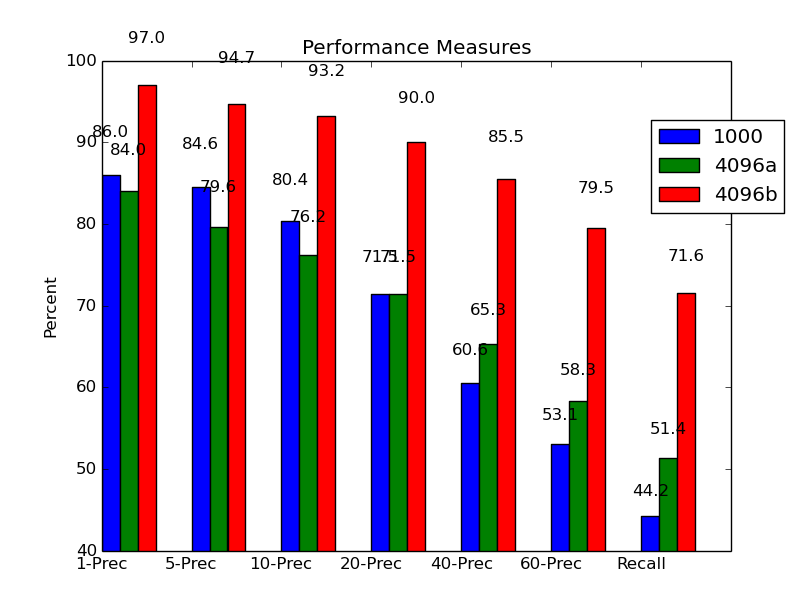
\includegraphics[width=9cm]{Figures/results/res-wang1.png}
&
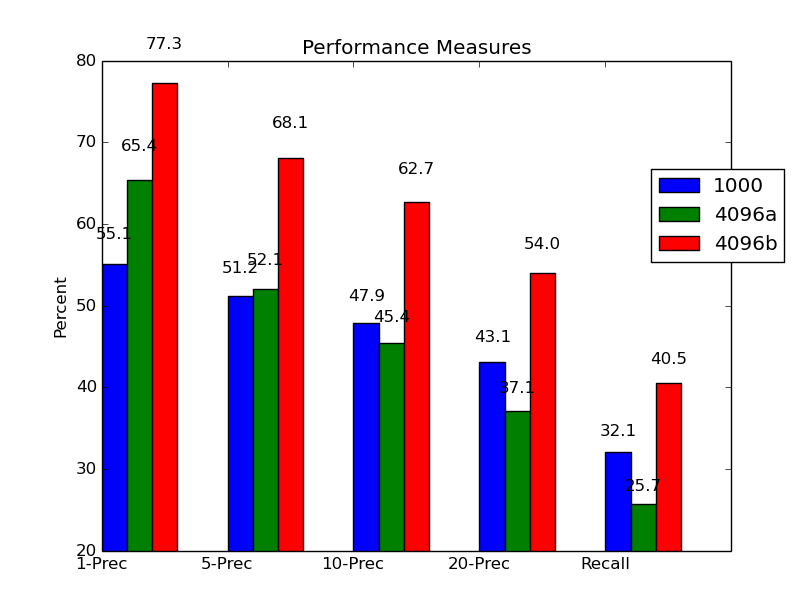
\includegraphics[width=9cm]{Figures/results/res-caltech1.png}\\
WANG & Caltech-101\\
\end{tabular}
\caption[comp7]{Résultats obtenus sur les deux bases.}
\end{figure}

	Il est clair que la représentation sémantique profonde de la couche 4096b dépasse de loin la représentation sémantique non profonde de la couche 4096a mais aussi la représentation en étiquette de la couche Soft-max 1000.

%Cette l'avant dernière couche du ConvNets, elle se trouve donc entre les deux couches précédemment utilisées. C'est une couche entièrement connectée qui contient 4096 neurones.
%Cette couche ajoute un traitement plus avancé des connaissances acquises de la couche qui la précède (4096a) mais elle est moins spécialisé que la dernière couche (1000 neurones par classes)
%SUPPOSITION: Rassembler les informations sémantiques obtenus des convolutions et de la couche précédente sans être classifiées en 1000 classes.


%\section{Sur quoi se base notre approche ?}
\section{La description sémantique}

	Pour expliquer les résultats que nous avons obtenus dans les trois approches décrites précédemment, nous devons comprendre ce qu'il se passe dans le réseau à convolution. Jusqu’à dernièrement, il n'y avait pas beaucoup de preuves sur ce qui se passait durant l'apprentissage, ce qui n’était pas satisfaisant d'un point de vue scientifique.

	L'approche de Matthew Zeiler [Zei et al. 14] nous a permis de trouver une théorie bien fondée pour expliquer l'apprentissage qu'effectuent les réseaux à convolution dans les parties contenant les piles de convolutions. Il montre dans sa recherche au fur et à mesure de la phase d'apprentissage, comment les valeurs des différents masques de convolutions changent et finissent à la fin par se spécialiser en apprenant à reconnaître un motif précis.
	
	Les filtres des premières couches de convolutions apprennent à reconnaître des motifs très simples par exemple: des traits, des coins, etc.	Les motifs deviennent de plus en plus complexes plus on avance à travers les couches de convolutions, jusqu'à arriver aux filtres de convolution des couches les plus profondes du réseau, qui apprennent à reconnaître des motifs beaucoup plus complexes en combinant les résultats des couches de convolution précédentes. Ces motifs complexes représenterons l'information sémantique que les réseaux à convolution reconnaissent.
Ainsi, on découvre qu'un réseau à convolution imite finalement bien le comportement observé dans le cerveau.

\subsection{Réseau à déconvolution}

	Matthew Zeiler réalise donc deux architectures, la première est un réseau à convolution qu'il a implémenté en se basant sur LeNet de LeCun [LeCun et al. 89] et AlNet de Krizhevsky [Kri et al. 12], comme le montre la figure suivante:

\begin{figure}[H]
	\centering
		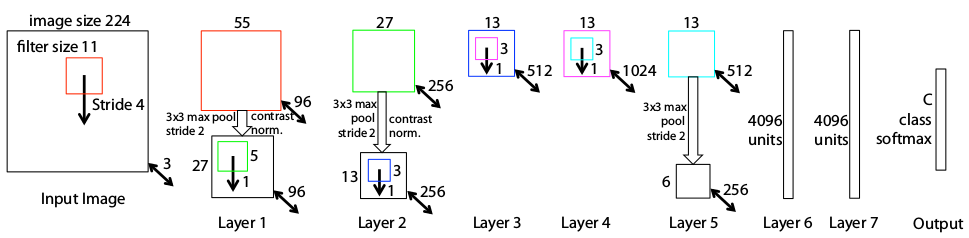
\includegraphics[width=5in]{Figures/arch.png}
	\caption[Res]{Architecture utilisée pour le conv net. [Zei et al. 14]}
	\label{fig:Electron}
\end{figure}

	Il a entraîné ce réseau à convolution sur la base d'images de ILSVRC-2012. Il a utilisé la Cross-Entropy pour le calcul d'erreur. L’entraînement fut effectué par descente du gradient avec des mini-batch d'une taille de 128 images, un Learning-Rate de 0.01 et un dropout sur les dernières couches d'une valeur de 0,5. Les poids furent initialisés à 0.01 et les biais à 0.

	La deuxième architecture que Matthew Zeiler a proposée dans son travail, offre une nouvelle manière de retracer les activités des caractéristiques détectées jusqu'à arriver vers les pixels qui les ont activés. Cette architecture s'intitule: \textit{réseaux de déconvolution}, ces derniers reprennent la même architecture que le réseau à convolution de la première architecture, mais d'une manière inverse. Ils effectuent dans l'ordre suivant ces étapes:

\begin{enumerate}
\item \textbf{Unpooling}: Le max-pooling qui est généralement utilisé dans les réseaux à convolution n'est pas inversible. L'Unpooling essaye d'approximer l'inverse du max-pooling, l’idée est donc de sauvegarder l'emplacement du maximum pour chaque région au moment de l'application d'un max-pooling. Comme le montre la figure suivante:

\begin{figure}[H]
	\centering
		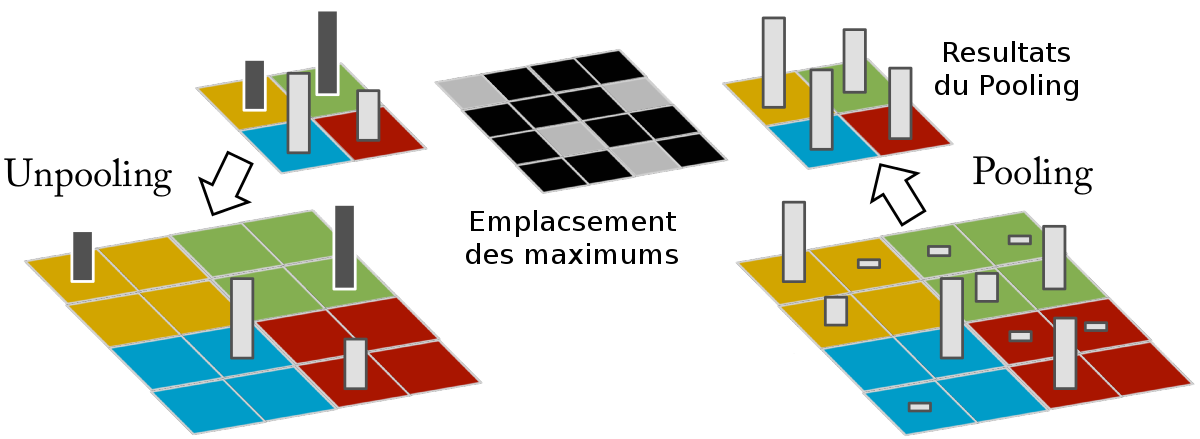
\includegraphics[width=5in]{Figures/unpooling.png}
	\caption[Res]{Schéma descriptif du unpooling. [Zei et al. 14]}
	\label{fig:Electron}
\end{figure}

\item \textbf{Rectification}: Elle s'effectue à travers l'application de la fonction de non-linéarité "ReLu", la rectification ne fait que prendre le maximum entre la valeur en entrée de la fonction et 0 pour garder seulement les résultats positifs, les négatifs deviendront des zéros.

\item \textbf{Filtrage}: la dernière étape est d'appliquer l'opération inverse des filtres (matrices) de convolution. Elle est considérée comme étant la transposée des filtres (matrices) de convolution apprises.
\end{enumerate}

\subsection{Visualisation des caractéristiques}

	Après avoir implémenté le réseau à déconvolution, Zeiler passe à la tâche de visualisation où il tente de donner un sens à l'apprentissage qu'effectue un réseau à convolution, en d'autres termes: montrer ce que chaque masque de convolution détecte. L'approche est donc de tenter de trouver les zones d'images en entrée qui sont à l'origine de l'activation de chaque masque. 
	
	Pour des raisons de manque de temps, nous n'avons pas pu implémenter les réseaux à déconvolutions sur notre implémentation. Les résultats obtenus par Zeiler [Zei et al. 14] sont représentés sur la figure ci-dessous, elle représente le top-9 des zones qui causent le plus grand taux d'activation pour un masque donné.
 
\begin{figure}[H]
	\centering
		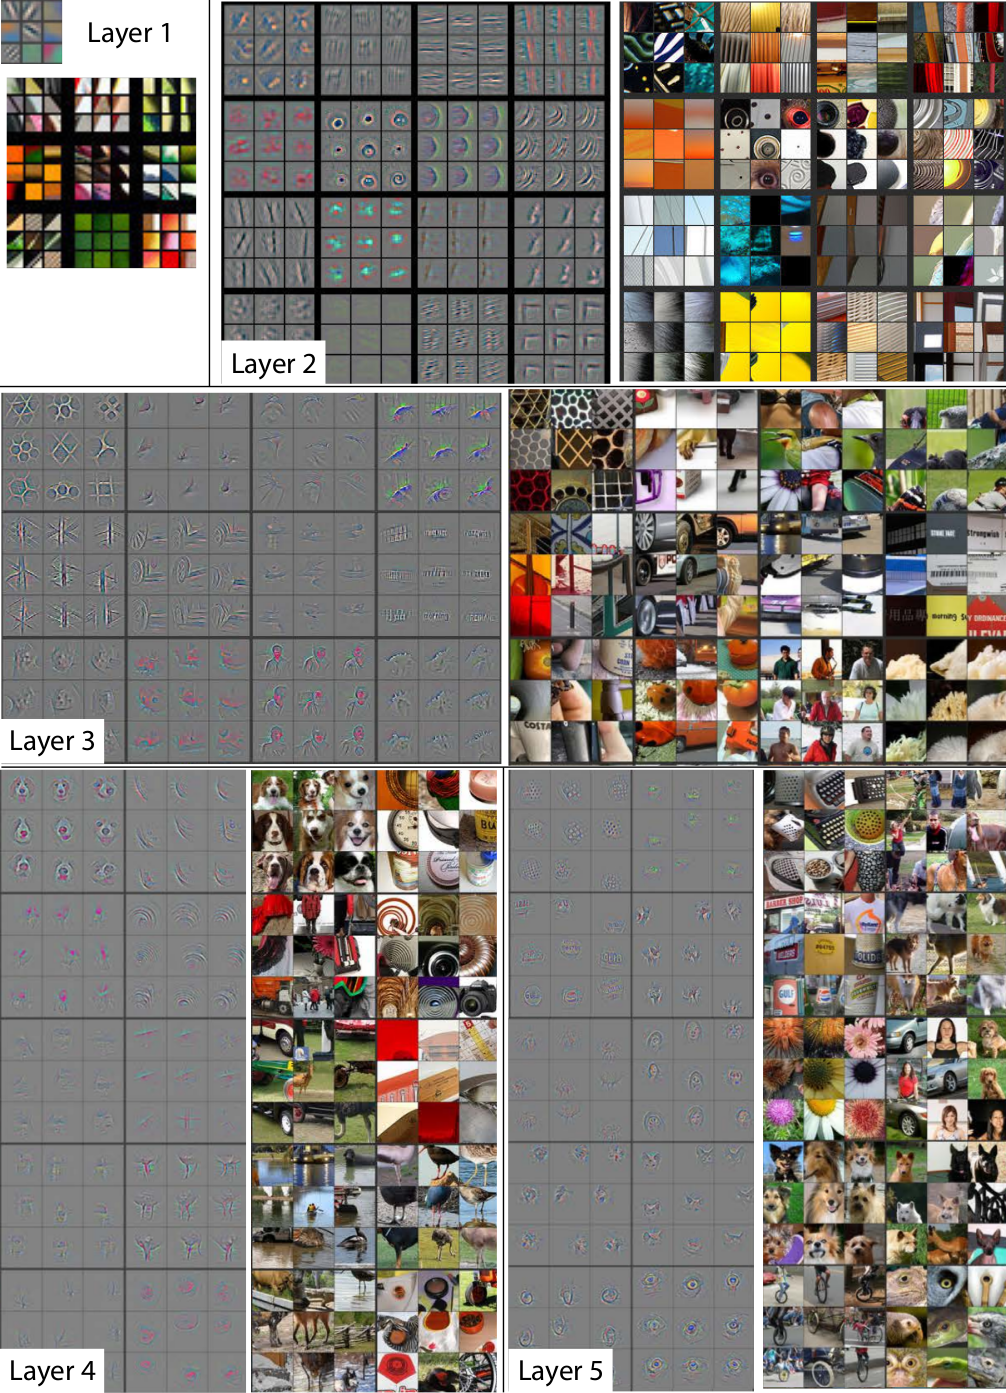
\includegraphics[width=5in]{Figures/visualisation.png}
	\caption[Res]{Visualisation des différences. [Zei et al. 14]}
	\label{fig:Electron}
\end{figure}


	On peut voir la nature hiérarchique de la reconnaissance, dans les premières couches, des formes basiques sont détectées (la détection de différents traits et lignes par la couche 1, différents types de coins par la couche 2). Ces formes basiques se combinent d'une couche à une autre pour arriver à des représentations plus complexes (des textures dans la couche 3), jusqu’à pouvoir reconnaître des objets plus significatifs dans les dernières couches (humain, chien, roue, fleur, etc.), c'est cette dernière reconnaissance qu'on qualifiera comme \textit{description sémantique}.

	Matthew Zeiler [Zei et al. 14] observe ainsi l’évolution des caractéristiques (features) reconnues durant l’entraînement et fait une analyse de sensibilité (sensitivity analysis). Puisque nous ne sommes pas certain que la détection se fait par rapport aux objets eux-mêmes et non pas à ce qu'ils ont autour (l'entourage des objets). Matthew Zeiler propose pour remédier à ce problème, de cacher certaines parties des images(avec des rectangles gris), les résultats des tests montrent que le taux de reconnaissance diminue d'une façon radicale, ce qui prouve donc que la détection se fait bien sur les objets eux mêmes et non leur entourage.\\

	Nous pouvons donc assumer qu'au final, la représentation retournée par le réseau est bien une représentation sémantique du contenu de l'image, elle décrit donc d'une certaine façon ce contenu. C'est cette représentation qui sera traduite en étiquettes (1000 classes) à travers la dernière couche Soft-max. Cette représentation force le réseau à utiliser des termes (étiquettes) bien précis pour exprimer ce qu'il a appris, c'est pour cette raison qu'on retrouve donc de meilleurs résultats lors de l'utilisation des sorties de l'avant dernière couche (4096b) où les concepts appris sont encore libres de cette contrainte. Enfin, plus les représentations sont traitées en profondeur, plus elles sont significatives, et plus le réseau apprend des concepts plus complexes. C'est comme cela que sont expliqués les résultats pas très bons de l'avant avant dernière couche (4096a).
	% (on remarque que les résultats de la couche de Soft-max (1000) se rapproches de celle de (4096a))

\section{Description sémantique avec les Autoencoders}
	Après avoir décrit ce qu'est la description sémantique d'une image, nous nous sommes intéressés dans nos approches suivantes à l'utilisation des Deep Autoencoders, en les appliquant sur les descriptions sémantiques que nous avons obtenus à partir du réseau à convolution que nous avons utilisé. Pour cela, nous avons choisi de prendre comme description sémantique celle de la couche 4096b (vu les bons résultats obtenus), qu'on essayera d'améliorer avec l'ajout des Deep Autoencoders.
	Les Deep Autoencoders que nous avons implémentés auront pour but de créer une représentation compressée des 4096 valeurs de la couche 4096b en seulement 1000 valeurs. Le choix de la valeur 1000 a été fait pour comparer entre les performances de la représentation par étiquette de la couche Soft-max 1000 et la représentation sémantique compressée de la couche 4096b avec les Deep Autoencoders.
	
	Comme pour un réseau de neurones classique, les Deep autoencoders doivent être entraînés sur une base d'exemples. Nous avons utilisé une nouvelle base d'images qui est IAPR TC-12 [Gru et at. 06] contenant 20000 images différentes. Nous avons choisi cette base d'images pour ne pas obtenir des résultats biaisés lors des calculs des ressemblances entre les images et avoir une meilleure généralisation. De cette manière, les Deep Autoencoders que nous avons implémentés créeront des représentations compressées des images des bases WANG et Caltech-101, en ayant appris à faire cela sur une toute autre base qui est IAPR TC-12.
	
	Chacune de nos architectures des autoencoders que nous avons implémentée ont été entraînées pendant plusieurs heures, entre 7 heures et 10 heures pour chaque architecture, pour un nombre d'epoch de 1000, un learning-rate de 0.1 et une taille de batch de 20.

\subsection{Autoencoder 4x1x4} 
	Nous avons implémenté notre première architecture de Deep Autoencoder de sorte à obtenir une description compressée de la couche sémantique 4096b en 1000 valeurs seulement. Nous avons donc choisi une architecture très simple, comme le montre la figure suivante:

\begin{figure}[H]
	\centering
		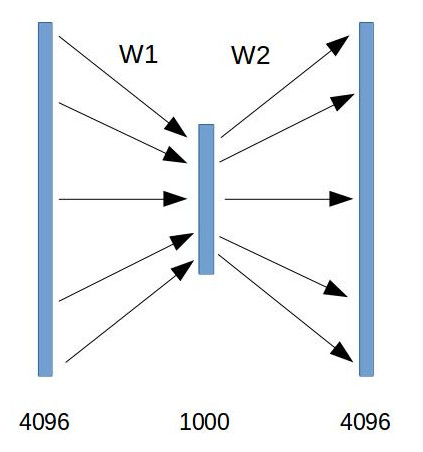
\includegraphics[width=2.5in]{Figures/ae/414.jpg}
	\caption[An Electron]{Architecture Autoencoder 4x1x4.}
	\label{fig:Electron}
\end{figure}

	Cette architecture a pour entrée une couche de 4096 valeurs qui contiendra la représentation sémantique 4096b d'une image, une couche cachée de 1000 valeurs où le Deep Autoencoder créera une représentation compressée des 4096 valeurs, et finalement la couche de sortie de 4096 valeurs où le Deep Autoencoder essayera de reconstruire l'entrée de 4096 valeurs à partir des 1000 valeurs compressées. On notera cette architecture en \textbf{Autoencoder 4x1x4}. Les résultats des mesures de performances que nous avons obtenus sont comme suit:
	

\begin{table}[H]
\begin{center}
\begin{tabular}{|c|c|c|c|c|c|c|c|}
\hline
	Mesure & 1-Préc & 5-Préc & 10-Préc & 20-Préc & 40-Préc & 60-Préc & Rappel\\
\hline
	WANG & 0.925 & 0.915 & 0.888 & 0.853 & 0.784 & 0.715 & 0.637\\
\hline
	Caltech-101 & 0.524 & 0.429 & 0.369 & 0.304 & - & - & 0.216\\
\hline
\end{tabular}
\end{center}
\caption{Résultats obtenus avec l'Autoencoder 4x1x4.}
\end{table}

	Nous remarquons que les résultats pour la base WANG ne sont pas meilleurs que ceux obtenus avec la représentation sémantique profonde de la couche 4096b, mais sont quand même meilleurs que ceux de la représentation sémantique non profonde de la couche 4096a, mais surtout meilleurs que la représentation par étiquette de la couche Soft-max 1000.
	Par contre pour la base d'images Caltech-101 ce n'est pas le même cas, la représentation avec l'autoencoder 4x1x4 ne donne pas de meilleurs résultats par rapport à toutes les autres approches précédentes.
	Comme les résultats ne sont pas les mêmes entre les deux bases d'images que nous avons testées, nous allons essayer d'autres architectures de Deep Autoencoder.


%Application d'un réseau d'autoencoder sur les valeurs de la couche 4096b, ce sera un apprentissage qui aura pour but de codifier (convertir) les 4096 valeurs en seulement 1000 valeurs. Ce réseau à une architecture très simple qui est comme suit: 4096 neurones dans la couche d'entrée, 1000 neurones dans la couche cachée et 4096 neurones dans la couche de sortie.
%SUPPOSITION: Obtenir de meilleurs résultats que la première approche qui utilise la dernière couche de 1000 neurones par classe.


\subsection{Autoencoder 4x2x1x2x4} 

	Comme l'approche précédente, la prochaine architecture de Deep Autoecnoder que nous avons implémenté aura pour but d'obtenir une description compressée de la couche sémantique 4096b en 1000 valeurs. Cette architecture sera par contre plus profonde que la précédente, comme le montre la figure suivante:

\begin{figure}[H]
	\centering
		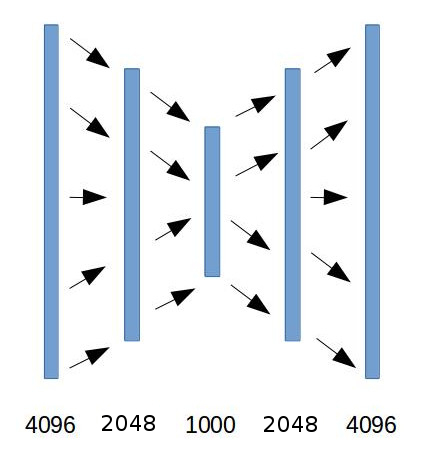
\includegraphics[width=2.5in]{Figures/ae/42124.jpg}
	\caption[An Electron]{Architecture Autoencoder 4x2x1x2x4.}
	\label{fig:Electron}
\end{figure}

	Cette architecture est un Deep Autoencoder plus profond que le précédent. La couche d'entrée aura 4096 valeurs qui seront la représentation sémantique de la couche 4096b, la même chose pour la couche de sortie où on essayera de reconstruire l'entrée du réseau. Par contre, nous avons trois couches cachées contrairement à une seule couche cachée seulement pour l'architecture précédente. La première couche cachée contiendra 2048 valeurs, la deuxième 1000 valeurs, et la troisième 2048 valeurs. Cette architecture aura comme objectif de compresser les 4096 valeurs en 2048 valeurs ensuite en 1000 valeurs, et puis reconstruire les 2048 valeurs à partir des 1000, et reconstruire les 4096 valeurs à partir des 2048 de la troisième couche. On notera cette architecture en \textbf{Autoencoder 4x2x1x2x4}. Les résultats que nous avons obtenus sont comme suit:

\begin{table}[H]
\begin{center}
\begin{tabular}{|c|c|c|c|c|c|c|c|}
\hline
	Mesure & 1-Préc & 5-Préc & 10-Préc & 20-Préc & 40-Préc & 60-Préc & Rappel\\
\hline
	WANG & 0.95 & 0.934 & 0.925 & 0.907 & 0.872 & 0.826 & 0.756\\
\hline
	Caltech-101 & 0.772 & 0.688 & 0.636 & 0.556 & - & - & 0.420\\
\hline
\end{tabular}
\end{center}
\caption{Résultats obtenus avec l'Autoencoder 4x2x1x2x4.}
\end{table}

	Pour les deux bases WANG et Caltech-101, nous avons obtenus des résultats presque similaires entre la couche 4096b et cette architecture Autoencoder 4x2x1x2x4. La représentation sémantique de 4096b donne de meilleures performances lors de la recherche d'images avec les Précision 1-Préc, 5-Préc et 10-Préc. Par contre pour le reste des mesures surtout le Rappel, l'architecture Autoencoder 4x2x1x2x4 est un peu meilleure que celle de 4096b.
	
	La différence entre les deux approches est qu'avec celle de 4096b nous comparons 4096 valeurs, quand à la représentation Autoencoder 4x2x1x2x4 nous ne comparons que 1000 valeurs seulement vu que c'est une représentation compressée.


%Cette approche utilise une autre architecture d'un réseau autoencoder qui est plus profond que le précédent. Son architecture est comme suit : Une couche d'entrée de 4096 neurones, trois couches cachées ayant dans l'ordre 2048, 1000 et 2048 neurones et finalement la couche de sortie de 4096 neurones.
%SUPPOSITION: Obtenir un meilleur taux d'apprentissage que l'autoencoder précedent.


\subsection{Denoising Autoencoder 4x1x4}
	En regardant les résultats des deux architectures de Deep Autoencoder, nous avons remarqué qu'il n'y avait pas vraiment d'amélioration ou seulement une légère amélioration. Au lieu de changer d'architecture de Deep Autoencoder, nous avons pensé à implémenter un autre type de Deep Autoencoder que sont les Deep Denoising Autoencoder. L'architecture d'un Deep Denoising Autoencoder ressemble à l'architecture d'un Deep Autoencoder, c'est la manière d'envoyer les valeurs en entrée qui change, comme le montre la figure suivante:

\begin{figure}[H]
	\centering
		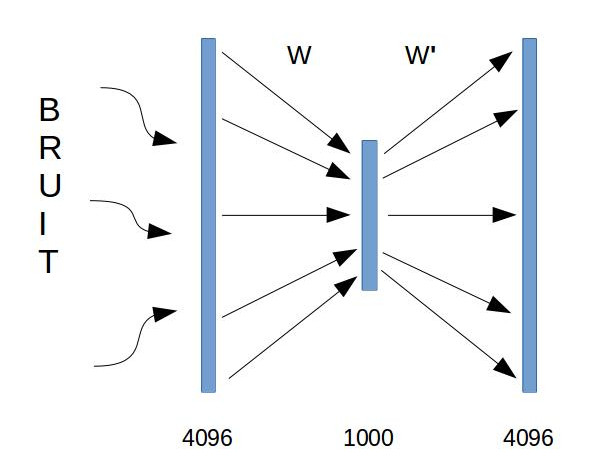
\includegraphics[width=3in]{Figures/ae/denoising.jpg}
	\caption[An Electron]{Architecture Deep Denoising Autoencoder 4x1x4.}
	\label{fig:Electron}
\end{figure}

	Cette architecture ressemble donc à l'architecture Autoencoder 4x1x4, comme nous le remarquons chaque donnée en entrée va être corrompue avec un certain taux de corruption. Donc les valeurs en entrée du réseau seront les valeurs de la couche sémantique 4096b, mais qui auront des valeurs modifiées à un certain taux. Le Deep Denoising Autoencoder que nous avons implémenté aura pour but dans ce cas de reconstruire à partir des 4096 valeurs corrompues, les 4096 valeurs non corrompues.
	
	Notre implémentation de Deep Denoising Autoencoder 4x1x4  a un taux de corruption de 30\% donc $4096 * \dfrac{30}{100} = 1228$ valeurs corrompues, les résultats obtenus sont comme suit:


\begin{table}[H]
\begin{center}
\begin{tabular}{|c|c|c|c|c|c|c|c|}
\hline
	Mesure & 1-Préc & 5-Préc & 10-Préc & 20-Préc & 40-Préc & 60-Préc & Rappel\\
\hline
	WANG & 0.965 & 0.95 & 0.936 & 0.926 & 0.905 & 0.870 & 0.808\\
\hline
	Caltech-101 & 0.813 & 0.748 & 0.705 & 0.638 & - & - & 0.511\\
\hline
\end{tabular}
\end{center}
\caption{Résultats obtenus avec le Denoising Autoencoder 4x1x4.}
\end{table}

	Les résultats de cette approche sont les meilleurs de tous les résultats des approches précédentes, que ce soit pour base WANG ou pour la base Caltech-101. Une amélioration des performances allant jusqu'à 10\% dans le Rappel par rapport à l'approche de la couche 4096b.
	Nous pouvons donc déduire que notre approche avec le Deep Denoising Autoencoder a pu construire une représentation compressée de 4096b en seulement 1000 valeurs, où elle garde seulement les informations utiles de la représentation sémantique 4096b, et cela améliore nettement la comparaison des images et donc la recherche d'image par le contenu. 


%Nous avons tester un autoencoder plus complexe. C'est la même architecture que l'autoencoder 4x1x4, mais avec un taux de corruption de 30\% et moins de paramètre pour éviter au maximum le sur-apprentissage.
%SUPPOSITION: Forcer un apprentissage plus significatif et réaliste.

\subsection{Résultats}

	Les deux graphes suivants montrent une comparaison entre l'approche 4096b et ceux des différentes architectures d'Autoencoders que nous avons implémentées:

\begin{figure}[H]
\centering
\begin{tabular}{cc}
\centering

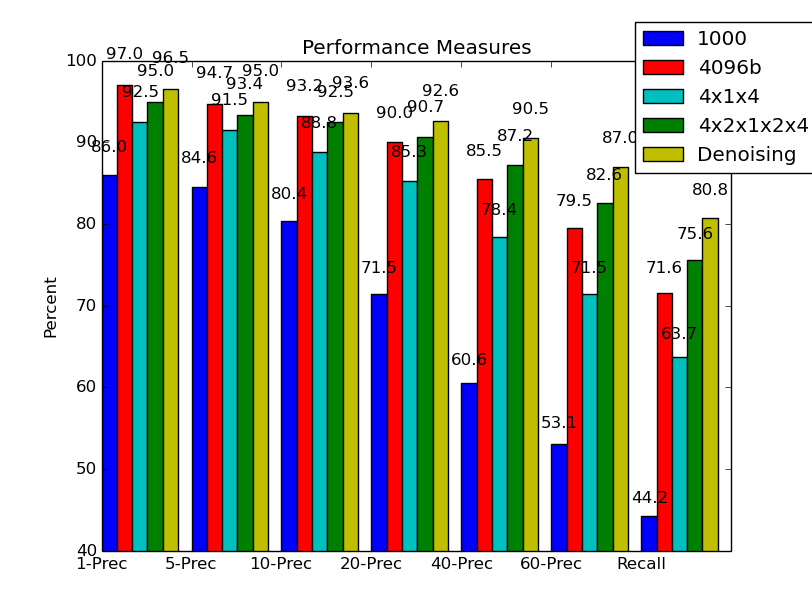
\includegraphics[width=9cm]{Figures/results/res-wang2b.png}
&
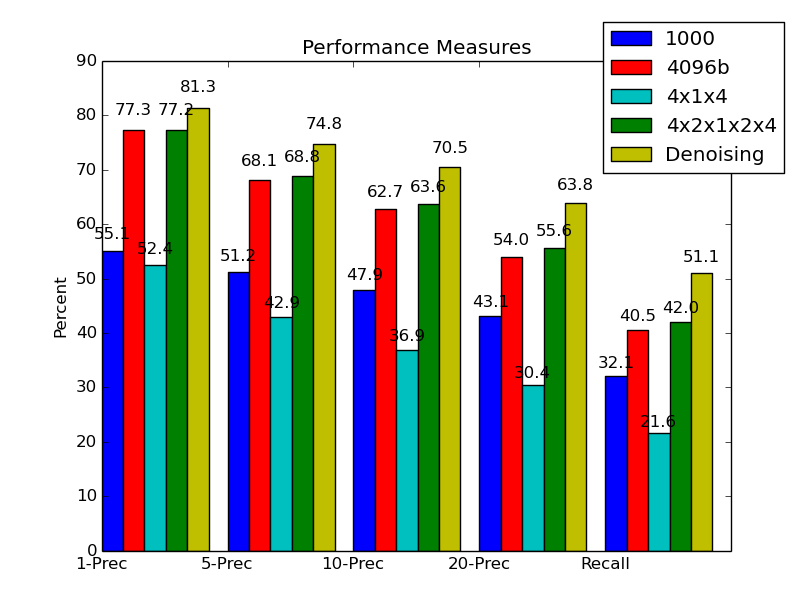
\includegraphics[width=9cm]{Figures/results/res-caltech2b.png}\\
WANG & Caltech-101\\
\end{tabular}
\caption[comp7]{Résultats avec Autoencoder obtenus sur les deux bases.}
\end{figure}

	Nous remarquons que les représentations compressées en 1000 valeurs des Autoecnoders donnent en général de meilleurs résultats que la couche Soft-max 1000, même si dans les deux cas les deux vecteurs ont une même taille. Donc la différence de performance entre les couches du réseau à convolutions (Soft-max 1000, 4096a et 4096b), n’était pas dû à la compression des espaces de représentation, mais à la différence du type d'information (sémantique ou étiquette) que contiennent ces couches, et aussi à la profondeur du traitement.
	
	Nos deux premières architectures d'Autoencoders qui sont Autoencoder 4x1x4 et 4x2x1x2x4 ne donnent pas de meilleurs résultats par rapport à l'approche 4096b, mais avec notre troisième architecture du Denoising Autoencoder, on remarque une très grande amélioration. Cela est dû à l'ajout des bruits (noises) qui rajoutent des contraintes supplémentaires au Denoising Autoencoder pour créer des représentations compressées plus efficaces. Ces résultats montrent la force des Deep Autoencoders.


\section{La force des Deep Autoencoders}
	En plus de réduire l'espace de représentation pour prouver que ce n'est pas finalement ce dernier qui influe sur les résultats, l'utilisation des Autoencoders a montré une amélioration considérable des résultats de recherches d'images.

	Pour comprendre pourquoi ceci s'est produit nous allons explorer plus en détail le fonctionnement de l'Autoencoder [Goo et al. 16]. L’idée est, comme expliqué précédemment dans le chapitre 2, que les données sont concentrées autour d'une partie d'un espace d'une dimension (appelée Variété ou Manifold) inférieure à celle de l'espace de représentation actuelle des données. L'objectif est de retrouver la structure de cette dimension réduite. Un Autoencoder effectue cela en faisant le compromis entre les deux contraintes suivantes:

\begin{enumerate}[i]
\item Apprendre une représentation \textit{h} d'un exemple en entrée \textit{x} (\textit{h} étant généralement d'une dimensionnalité plus inférieure) tel que \textit{x} peut être récupéré à partir de \textit{h} grâce à un décodeur, et ceci avec un minimum d'erreur. Si le \textit{x'} (reconstruit à partir \textit{x}) n'appartient pas à l'espace de données en entrée, la reconstruction n'est pas sensée donner de bons résultats.

\item Le deuxième point à satisfaire est l'ensemble de régularisations qui sont infligées à un Autoencoder et qui ont généralement pour but d’éviter le sur-apprentissage et permettre donc d'avoir une représentation plus générale.

\end{enumerate}


\begin{figure}[H]
	\centering
		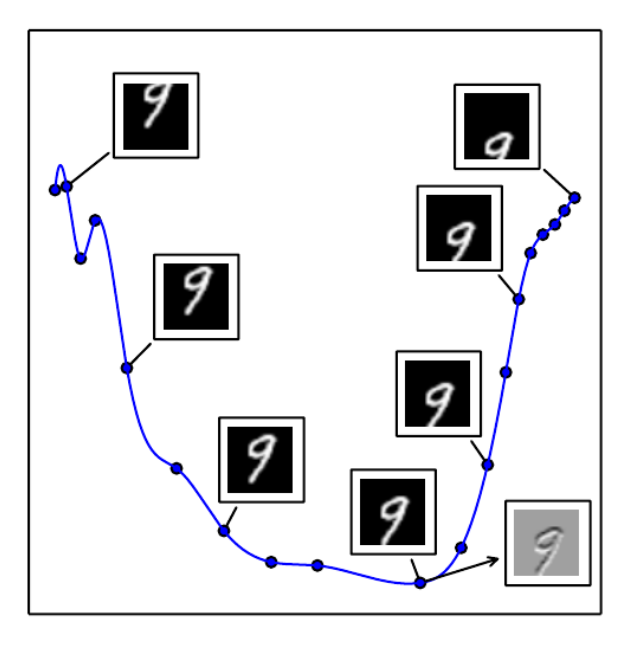
\includegraphics[width=3.5in]{Figures/manifold.png}
	\caption[Res]{Exemple d'une Variété à une dimension [Goo et al. 16] dans un espace de 784 dimensions des images de la base MNIST (28×28 pixels) [LeCun et al. 98]. Une image fut prise et déplacée verticalement de haut en bas. Le taux de déplacement vertical définit des coordonnées qui tracent une courbe. Pour la visualiser, cette dernière a été projetée vers un espace à 2 dimensions en utilisant PCA (Principal Component Analysis).}
	\label{fig:Electron}
\end{figure}


	Nous expliquons donc, dans notre cas, la hausse de niveau de précision dans la comparaison des images par le fait que les représentations sémantiques retenues par le réseau à convolution soient compressées par le codeur, il constitue dorénavant un moyen de résumer les représentations en les combinant d'une façon à en garder ce qu'il y a de plus essentiel.

Ensuite, les contraintes ajoutées au Denoising Autoencoder lui ont permis d'apprendre une compression plus générale et plus efficace, d’où ses résultats remarquables.


\section{Recherche avec descripteur d'image}
	Comme nous l'avons mentionné au début de ce chapitre, nos contributions aux techniques de recherche d'images par le contenu basée-exemple est de proposer des alternatives aux descripteurs usuels qui étaient utilisés pour calculer la ressemblance des images et les comparer entre elles. Nous avons ensuite montré la puissance des techniques de l'apprentissage profond et ce qu'ils peuvent donner comme résultats. Dans cette partie, nous allons rajouter des descripteurs de textures aux meilleures représentations que nous avons obtenues (4096b et Denoising Autoencoder). Pour les descripteurs de texture, nous avons choisi le Local Binary Pattern [Oja et al. 02] (Motifs Locaux Binaires) et les matrices de co-occurences GLCM [Har 79] (Grey Level Co-Occurences Matrix).

\subsection{4096b avec descripteur}
	Dans cette approche nous allons rajouter aux 4096 valeurs de la couche sémantique 4096b deux descripteurs, qui sont l'histogramme des motifs uniformes du Local Binary Pattern avec invariabilité aux rotations [Oja et al. 02], et les mesures suivantes des matrices de co-occurences [Har 79]: contraste, dissimilarité, homogénéité, énergie, corrélation, second moment angulaire.
	
	Les résultats obtenus sont représentés dans le tableau suivant: 

\begin{table}[H]
\begin{center}
\begin{tabular}{|c|c|c|c|c|c|c|c|}
\hline
	Mesure & 1-Préc & 5-Préc & 10-Préc & 20-Préc & 40-Préc & 60-Préc & Rappel\\
\hline
	WANG & 0.964 & 0.949 & 0.937 & 0.919 & 0.880 & 0.835 & 0.713\\
\hline
	Caltech-101 & 0.774 & 0.681 & 0.627 & 0.539 & - & - & 0.405\\
\hline
\end{tabular}
\end{center}
\caption{Résultats obtenus avec l'ajout des descripteurs de texture.}
\end{table}

	Les résultats que nous avons obtenus ressemblent beaucoup à ceux des résultats de la couche sémantique 4096b pour la base Caltech-101, et on remarque une légère amélioration de 2\% à 3\% dans certaines mesures de performances pour la base d'images WANG. On peut dire que l'ajout de descripteur n'a pas un impact important lors de la comparaison des images.


\subsection{Denoising Autoencoder avec descripteur}
	Nous allons dans cette approche prendre les mêmes valeurs de l'approche précédente qui sont les 4096 valeurs de la couche sémantique 4096b en plus de l'histogramme du Local Binary pattern et les mesures de matrices de co-occurences, ces valeurs seront données en entrée à une nouvelle architecture de Deep Denoising Autoencoder que nous avons implémenté qui est représentée sur la figure suivante:
	
\begin{figure}[H]
\centering
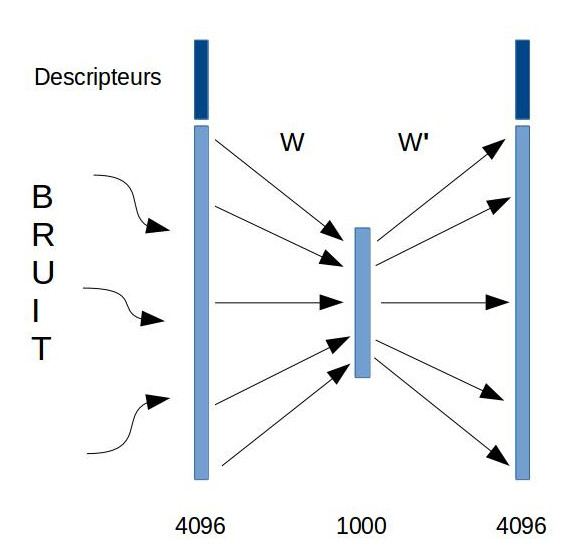
\includegraphics[width=3in]{Figures/ae/AE-Descripteur.jpg}
\caption[An Electron]{Architecture Denoising Autoencoder 4x1x4 avec descripteur.}
\label{fig:Electron}
\end{figure}

	Cette architecture a une couche d'entrée contenant les valeurs de la couche 4096b plus les valeurs des descripteurs mais avec un taux de corruption de 30\%, nous avons dans cette architecture une seule couche cachée qui a une taille de 1000 valeurs, et une couche de sortie qui devra reconstruire les 4096 valeurs plus les valeurs des descripteurs de textures tout en détectant les valeurs corrompues. Les résultats obtenus sont comme suit:

\begin{table}[H]
\begin{center}
\begin{tabular}{|c|c|c|c|c|c|c|c|}
\hline
	Mesure & 1-Préc & 5-Préc & 10-Préc & 20-Préc & 40-Préc & 60-Préc & Rappel\\
\hline
	WANG & 0.96 & 0.952 & 0.939 & 0.929 & 0.905 & 0.874 & 0.811\\
\hline
	Caltech-101 & 0.816 & 0.746 & 0.707 & 0.641 & - & - & 0.512\\
\hline
\end{tabular}
\end{center}
\caption{Résultats obtenus avec Denoising Autoencoder avec descripteurs de texture.}
\end{table}

	Ces résultats sont presque similaires aux résultats obtenus avec le Denoising Autoencoder sans descripteurs, nous remarquons par contre une très légère amélioration de 0.2\% à 0.3\% dans presque toutes les mesures de performances des deux bases d'images.
	

%avec descripteurs (SIFT,LBP,GLCM,formes,couleurs) : L'architecture de ce réseau ressemble un peu aux précédentes, sauf qu'au lieu de donner en entrée/sortie seulement les 4096 valeurs, on va leurs rajouter différents descripteurs. La combinaison de ses valeurs devra être codifié en 1000 valeurs dans la couche cachée.
 
%SUPPOSITION: On ne sait pas si les descripteurs "fabriqués à la main" vont aider à améliorer l'apprentissage ou bien non. Le cerveau n'effectue pas ce genre de calcul, mais l'architecture de l'ordinateur peut lui permettre d'exploiter ses différents descripteurs pour une meilleure reconnaissance.


\subsection{Résultats}
	Les deux graphes suivants montrent les résultats entre l'approche 4096b, le Denoising Autoencoder et les deux approches avec les descripteurs:
	
\begin{figure}[H]
\centering
\begin{tabular}{cc}
\centering

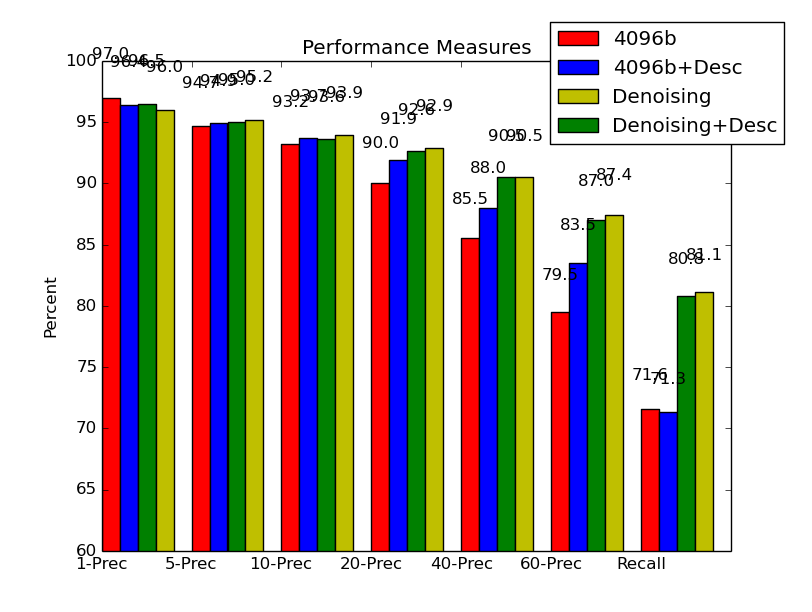
\includegraphics[width=9cm]{Figures/results/res-wang3.png}
&
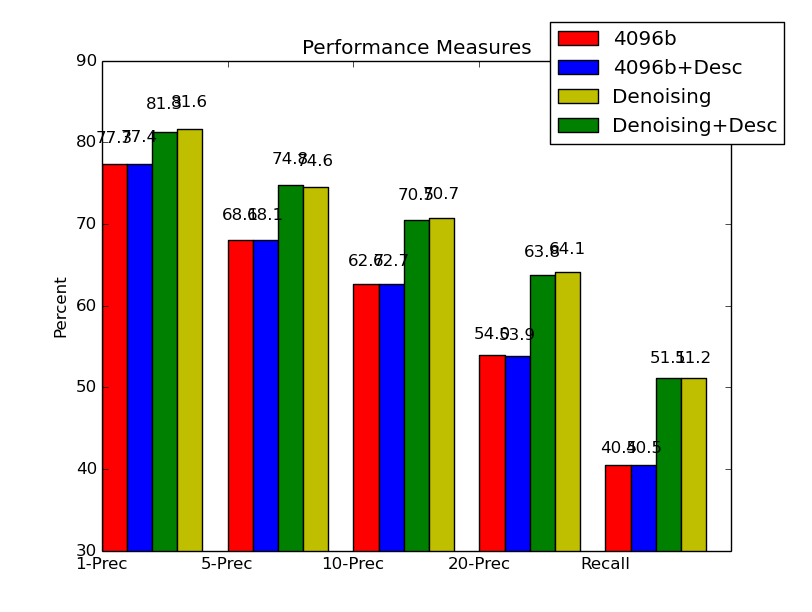
\includegraphics[width=9cm]{Figures/results/res-caltech3.png}\\
WANG & Caltech-101\\
\end{tabular}
\caption[comp7]{Résultats avec descripteurs obtenus sur les deux bases.}
\end{figure}
	
	Nous remarquons que l'ajout ou non de descripteurs aux représentations sémantiques n'affecte pas les résultats d'une manière considérable. Nous pouvons donc dire que nos représentations sémantiques de nos approches offrent de bonnes descriptions des images sans avoir besoins d'ajouter des descripteurs d'images.
On pourrait aussi dire que les informations d'une image qu'offrent les descripteurs sont déjà inclues dans la description sémantique de l'image.

\section{Comparaison avec d'autres systèmes CBIR}

	Dans cette partie nous allons comparer toutes nos approches qui sont la description sémantique de la couche 4096b, et la description du Denoising Autoencoder 4x1x4 sans descripteurs. Comme exemple de système de recherche d'image par le contenu, nous avons choisi deux systèmes de recherche qui sont FIRE [Des et al. 08] et LIRE [Lux et al. 13], parce-que ces deux systèmes ont utilisé des descripteurs traditionnels pour donner une description des images, et ont présenté les mesures de performances que leurs systèmes ont obtenus sur la base WANG [Li et Wan.,03][Wan et al.,01]. Parmi ces mesures de performances ils utilisent le taux d'erreur (événement inverse de la 1-Précision) pour comparer leurs différentes approches.
	
	Les résultats des deux systèmes LIRE et FIRE sont représentés dans les deux tableaux suivants:
	
	
\begin{table}[H]
\begin{center}
\begin{tabular}{|c|c|}
\hline
Descripteur & Taux d'erreur\\
\hline
color histogram & 0.169\\
LF SIFT global search & 0.372\\
LF patches histogram & 0.179\\
LF SIFT histogram & 0.256\\
inv. feature histogram (monomial) & 0.192\\
MPEG7: scalable color & 0.251\\
LF patches signature & 0.243\\
Gabor histogram & 0.305\\
32x32 image & 0.472\\
MPEG7: color layout & 0.354\\
Xx32 image & 0.559\\
Tamura texture histogram & 0.284\\
LF SIFT signature & 0.351\\
gray value histogram & 0.453\\
LF patches global & 0.429\\
MPEG7: edge histogram & 0.328\\
inv. feature histogram (relational) & 0.383\\
Gabor vector & 0.655\\
global texture feature & 0.514\\
\hline
\end{tabular}
\end{center}
\caption{Résultats du système FIRE. [Des et al. 08]}
\end{table}


\begin{table}[H]
\begin{center}
\begin{tabular}{|c|c|}
\hline
Descripteur & Taux d'erreur\\
\hline
Auto color correlogram & 0.171\\
CEDD & 0.178\\
Color histogram & 0.191\\
FCTH & 0.209\\
Gabor & 0.707\\
JCD & 0.177\\
Joint histogram & 0.196\\
JPEG coefficients histogram & 0.215\\
MPEG-7 color layout & 0.309\\
MPEG-7 scalable color & 0.462\\
MPEG-7 edge histogram & 0.401\\
SIFT BoVW & 0.687\\
Tamura & 0.601\\
\hline
\end{tabular}
\end{center}
\caption{Résultats du système LIRE. [Lux et al. 13]}
\end{table}

	Rappelons que la base WANG contient 1000 images (10 classes des 100 images), contrairement à notre algorithme de recherche d'image par le contenu où nous avons divisé la base WANG en deux parties (la première contenant 20\% des images et la deuxième le reste des 80\%), les approches des deux systèmes sont un peu différentes. Ils calculent le taux d'erreur pour les 1000 images et non pas 200 requêtes comme dans notre algorithme, pour cela ils prennent chaque image et ils la comparent avec les 999 autres images, si l'image la plus ressemblante appartient à la même classe, le taux d'erreur sera égal à 0 sinon à 1 dans le cas contraire.

	Le choix du taux d'erreur comme mesure pour comparer les différents modèles de recherche d'image par le contenu, est dû au fait que quand un utilisateur cherche les images ressemblantes à son image (à partir d'un smartphone par exemple), il s'intéresse généralement au top-5 des images ressemblantes, et principalement au top-1, donc il est plus important de donner les bonnes images pertinentes en premier que de retourner plusieurs images qui ne sont pas toutes forcément pertinentes.
	
	Nous avons donc implémenté un nouvel algorithme qui utilise la même manière de comparaison que les deux systèmes LIRE et FIRE (1 image requête comparée avec les 999 autres images), pour nous permettre de les comparer avec nos approches, les résultats sont comme suit:

\begin{table}[H]
\begin{center}
\begin{tabular}{|c|c|c|c|c|c|c|c|c|}
\hline
	Comp & 1000 & 4096a & 4096b & AE414 & AE42124 & Denosing & 4096b+Desc & Denoising+Desc\\
\hline
	\multicolumn{9}{|c|}{1-Précision}\\
\hline
	20\%-80\% & 0.86 & 0.84 & 0.97 & 0.925 & 0.95 & 0.965 & 0.97 & 0.96\\
\hline
	1-999 & 0.885 & 0.87 & 0.964 & 0.935 & 0.953 & 0.966 & 0.964 & 0.967\\
\hline
	\multicolumn{9}{|c|}{Rappel}\\
\hline
	20\%-80\% & 0.442 & 0.514 & 0.716 & 0.637 & 0.756 & 0.808 & 0.717 & 0.811\\
\hline
	1-999 & 0.413 & 0.520 & 0.713 & 0.641 & 0.758 & 0.806 & 0.713 & 0.807\\
\hline
\end{tabular}
\end{center}
\caption{Comparaison des mesures obtenues entre les deux manières de comparaison.}
\end{table}

	Avant de comparer nos résultats avec les bases LIRE et FIRE, nous allons d'abord comparer nos deux manières de comparaison de la base WANG que nous avons implémenté, nous remarquons que les 1-Précision et Rappels des deux manières de comparaison sont très similaires, avec une différence rare de 3\% au maximum. On peut donc dire que les mesures de performance sur une partie aléatoire d'une base d'image, sont approximativement les mêmes que les mesures sur la totalité de la base. Le tableau [Tableau 3.13] ci-dessous donne les valeurs des taux d'erreur avec la manière (1 avec 999) :

\begin{table}[H]
\begin{center}
\begin{tabular}{|c|c|c|c|c|c|c|c|c|}
\hline
	Mesure & 1000 & 4096a & 4096b & AE414 & AE42124 & Denosing & 4096b+Desc & Denoising+Desc\\
\hline
	1-Préc & 0.885 & 0.87 & 0.964 & 0.935 & 0.953 & 0.966 & 0.964 & 0.966\\
\hline
	Taux-Err & 0.115 & 0.13 & 0.036 & 0.065 & 0.047 & 0.034 & 0.036 & 0.034\\
\hline
\end{tabular}
\end{center}
\caption{Les mesures obtenues avec la nouvelle manière de comparaison (1 avec 999).}
\end{table}




	Nous allons comparer tous nos approches avec les descripteurs de LIRE et FIRE qui ont donné les plus petits taux d'erreur, color histogram pour FIRE et Auto color correlogram pour LIRE, les résultats sont présentés sur le graphe suivant:
	
\begin{figure}[H]
\centering
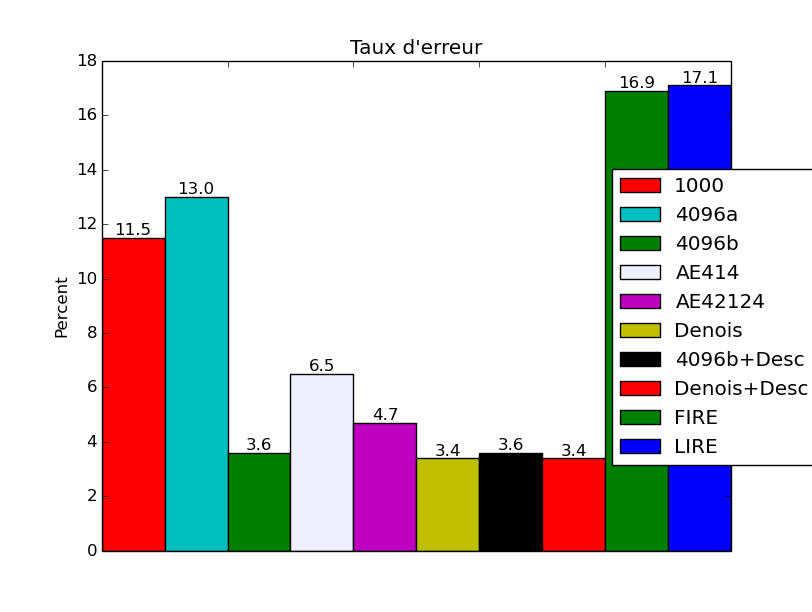
\includegraphics[width=5in]{Figures/results/res-wang5.png}
\caption[An Electron]{Comparaison de nos approches avec FIRE et LIRE.}
\label{fig:Electron}
\end{figure}
	
	Il est clair que les taux d'erreur de nos approches sont très largement petits par rapport à ceux des deux systèmes LIRE et FIRE, sauf pour les approches de la couche Soft-max 1000 (par étiquette) et la couche 4096a (sémantique mais non profonde). Cela confirme la puissance de la description sémantique profonde ainsi que la puissance des Deep Autoencoders. Nos techniques utilisées offrent donc une meilleure alternative aux descripteurs d'images traditionnels.
	
\section{Conclusion}

	Nous concluons ce chapitre en constatant que les méthodes d'apprentissage profond donnent effectivement des résultats très satisfaisants quand on les applique au problème de recherche d'image par le contenu.
	Les méthodes d'apprentissage profond que nous avons implémenté dans nos approches sont les réseaux à convolution (ConvNets) et les Deep Autoencoders, nous avons proposé une nouvelle approche pour décrire une image qui est la description sémantique, nous avons montré à quel point cette description est efficace et comment nous avons pu l'améliorer en utilisant des Deep Autoencoders.
	
	Comme les techniques d'apprentissage profond sont nouvelles et très variées, nos approches pourraient être développées et améliorées pour donner de meilleurs résultats en performance et en temps d’exécution. Nous allons dans le prochain chapitre, aborder les détails techniques de nos implémentations, ainsi qu'une visualisation concrète des exemples d'images retrouvées par notre système.
